\documentclass[conference]{IEEEtran}
\IEEEoverridecommandlockouts
\usepackage{standalone}
\usepackage{tikz} % O los paquetes que use tu figura
\usepackage{tikz-3dplot}
\usepackage{cite}
\usepackage{amsmath,amssymb,amsfonts}
\usepackage{algorithmic}
\usepackage{graphicx}
\usepackage{textcomp}
\usepackage{xcolor}
\usepackage{float}
\usepackage{booktabs}
\usepackage{url}

% -------Ajuste fino de espaçamento de figuras (IEEE-safe)-----------
%\setlength{\textfloatsep}{8pt plus 2pt minus 2pt}
%\setlength{\floatsep}{6pt plus 2pt minus 2pt}
%\setlength{\intextsep}{6pt plus 2pt minus 2pt}
%--------------------------------------------------------------------
\DeclareUnicodeCharacter{2060}{}

\def\BibTeX{{\rm B\kern-.05em{\sc i\kern-.025em b}\kern-.08em
    T\kern-.1667em\lower.7ex\hbox{E}\kern-.125emX}}

\begin{document}

\title{Pseudo-Brewster Angle–Guided Bistatic SAR Optimization for Subsurface Sensing}

\author{
\IEEEauthorblockN{
David Atencia Mondagón\IEEEauthorrefmark{1}\IEEEauthorrefmark{4},
Eder Carlos Fernandes\IEEEauthorrefmark{1}\IEEEauthorrefmark{5},
Everton Gomede\IEEEauthorrefmark{2}\IEEEauthorrefmark{6},\\
João Roberto Moreira Neto\IEEEauthorrefmark{3}\IEEEauthorrefmark{7},
Hugo Enrique Hernández-Figueroa\IEEEauthorrefmark{1}\IEEEauthorrefmark{8}
}

\vspace{2pt}
\rule{0.0\linewidth}{0.4pt}
\vspace{4pt}

\IEEEauthorblockA{\IEEEauthorrefmark{1}State University of Campinas (UNICAMP), Campinas/SP 13083-852, Brazil}
\IEEEauthorblockA{\IEEEauthorrefmark{2}University of British Columbia (UBC), Vancouver/BC V6T 1Z4, Canada}
\IEEEauthorblockA{\IEEEauthorrefmark{3}Radaz S.A., São José dos Campos/SP 02047-901, Brazil}

\vspace{4pt}
\IEEEauthorblockA{
\IEEEauthorrefmark{4}david.mondagon@embraer.com.br,
\IEEEauthorrefmark{5}e208418@dac.unicamp.br,
\IEEEauthorrefmark{6}everton.gomede@ubc.ca, \\
\IEEEauthorrefmark{7}tech@radaz.com.br,
\IEEEauthorrefmark{8}hugo@unicamp.br
}
}

\maketitle

\begin{abstract}
This paper presents a physics-guided optimization framework for bistatic synthetic aperture radar (SAR) data acquisition aimed at subsurface sensing applications. The proposed approach integrates pseudo-Brewster-angle-based flight planning with receiver positioning to improve electromagnetic transmission through the air-ground interface in lossy dielectric media. A QGIS-based flight-planning tool was developed to generate bistatic drone trajectories conditioned on pseudo-Brewster-angle constraints and integrated with a drone-borne multi-band SAR system. Receiver placement is formulated as a multi-start optimization problem with physically motivated initialization strategies derived from electromagnetic transmission theory. Simulations conducted at 400 MHz indicate that pseudo-Brewster-guided bistatic geometries achieve the highest average received power (-70.11 dBm), compared with the perpendicular (-72.99 dBm) and opposite (-72.30 dBm) configurations. All reported values are averages across multiple target configurations and initialization seeds. The results indicate that explicitly incorporating electromagnetic transmission physics into bistatic SAR geometry design can yield measurable coupling gains in simulations.
\end{abstract}

\begin{IEEEkeywords}
Bistatic SAR, Pseudo-Brewster Angle, Receiver Optimization, Flight Planning, Subsurface Sensing
\end{IEEEkeywords}

\section{Introduction}

Subsurface investigation at depths of hundreds of meters remains a significant challenge for conventional radar systems \cite{daniels_gpr}. Ground-penetrating radar (GPR) techniques are typically limited to penetration depths of only a few tens of meters due to electromagnetic attenuation, whereas emerging applications such as mineral exploration, archaeological surveys, and groundwater detection demand deeper, more reliable sensing capabilities \cite{Soil}.

Bistatic radar systems, where transmitter and receiver are spatially separated, offer significant potential for enhanced penetration capabilities \cite{cherniakov_bistatic}. However, the effectiveness of these systems critically depends on the electromagnetic coupling efficiency at the air-ground interface, which is highly sensitive to the angle of incidence at lossy dielectric interfaces.
The pseudo-Brewster angle maximizes electromagnetic transmission in lossy media \cite{mcmichael_brewster} and, when incorporated into system design, provides a physics-based criterion for improving subsurface sensing configurations.

The proposed system integrates: (1) pseudo-Brewster-angle-based flight planning, (2) bistatic receiver optimization, and (3) an integrated drone-borne SAR platform. This work contributes an optimization workflow that integrates electromagnetic theory, mission planning, and SAR acquisition to support improved acquisition conditions for subsurface tomography processing.

This work reformulates bistatic SAR acquisition design from a geometry-driven heuristic into a physics-constrained optimization problem, in which electromagnetic transmission at the air–ground interface is explicitly embedded into trajectory planning and receiver positioning.

\section{Related Work and Theoretical Foundation}

This section reviews the electromagnetic principles underlying pseudo-Brewster-angle optimization in bistatic SAR systems and summarizes related work that motivates its use in subsurface sensing.

\subsection{Pseudo-Brewster Angle in Lossy Media}

The fundamental theory governing maximum transmission at interfaces for media with complex permittivity has been established for ground-penetrating radar applications. While the classical Brewster angle does not exist in lossy soils, a pseudo-Brewster angle that depends on complex permittivity (real and imaginary parts) provides practical optimization guidance \cite{mcmichael_brewster}.

For lossy media, the pseudo-Brewster angle minimizes reflection and maximizes transmission efficiency \cite{mcmichael_brewster}. This angle varies primarily with soil moisture and frequency, making it an important parameter for mission planning in subsurface sensing applications.

\subsection{Bistatic Radar for Subsurface Sensing}

Recent drone-borne SAR studies in P/L/C bands demonstrate feasibility for soil-moisture mapping and shallow subsurface anomaly detection with linear and helical trajectories \cite{ore_soil_moisture}.

The bistatic radar equation for subsurface targets must account for electromagnetic wave transmission through multiple media, including refraction and attenuation at the air–ground interface, as expressed in Eq.~\ref{eq:bistatic_radar}:

\begin{equation}
P_r = \frac{P_t G_t G_r \sigma T_{tx} T_{rx} \lambda^2}{(4\pi)^3 R_1^2 R_2^2 R_3^2 R_4^2}
\label{eq:bistatic_radar}
\end{equation}

where $P_t$ denotes the transmitted power, $G_t$ and $G_r$ are the transmitter and receiver antenna gains, respectively, $\sigma$ represents the radar cross section of the subsurface target, $T_{tx}$ and $T_{rx}$ are the power transmittance coefficients at the air–ground interface for the transmit and receive paths, $\lambda$ is the operating wavelength, and $R_1, R_2, R_3, R_4$ denote the individual propagation path segments illustrated in Figure~\ref{fig:bistatic_geometry}.

\begin{figure}[ht]
\centering
\scalebox{0.6}{% Figura 1: Geometría del sistema bistático
\documentclass[border=5pt]{standalone}
\usepackage{tikz}
\usepackage{tikz-3dplot}
\usetikzlibrary{arrows.meta, decorations.pathreplacing, calc} % <-- ADICIONAR calc

\begin{document}
\tdplotsetmaincoords{70}{110}

\begin{tikzpicture}[tdplot_main_coords, scale=0.8]

% Definir puntos
\coordinate (Tx) at (2, 4, 3);
\coordinate (Rx) at (-3, -2, 3);
\coordinate (Target1) at (0, 0, -2);
\coordinate (Target2) at (1, 1, -2);
\coordinate (Surface1) at (0.8, 1.6, 0);
\coordinate (Surface2) at (-0.6, -0.4, 0);

% Plano del suelo
\fill[gray!20, opacity=0.5] (-4,-4,0) -- (4,-4,0) -- (4,4,0) -- (-4,4,0) -- cycle;
\draw[gray] (-4,-4,0) -- (4,-4,0) -- (4,4,0) -- (-4,4,0) -- cycle;

% Subsuelo
\fill[brown!30, opacity=0.3] (-4,-4,-3) -- (4,-4,-3) -- (4,4,-3) -- (-4,4,-3) -- 
                              (-4,-4,0) -- (4,-4,0) -- (4,4,0) -- (-4,4,0) -- cycle;

% Transmisor
\draw[blue, thick] (Tx) circle (0.15);
\fill[blue] (Tx) circle (0.1);
\node[above, blue] at (Tx) {Transmitter};

% Receptor
\draw[red, thick] (Rx) circle (0.15);
\fill[red] (Rx) circle (0.1);
\node[above, red] at (Rx) {Receiver};

% Targets
\foreach \target in {Target1, Target2} {
    \draw[black, thick] (\target) circle (0.1);
    \fill[black] (\target) circle (0.08);
}
\node[below] at (Target1) {Target 1};
\node[below] at (Target2) {Target 2};

% Trayectorias de rayos
% Tx → Surface1 → Target1
\draw[blue, thick, ->] (Tx) -- (Surface1);
\draw[blue, thick, dashed, ->] (Surface1) -- (Target1);

% Target1 → Surface2 → Rx
\draw[red, thick, dashed, ->] (Target1) -- (Surface2);
\draw[red, thick, ->] (Surface2) -- (Rx);

% Etiquetas de distancias
\node[midway, above] at ($(Tx)!0.5!(Surface1)$) {$R_1$};
\node[midway, right] at ($(Surface1)!0.5!(Target1)$) {$R_2$};
\node[midway, left] at ($(Target1)!0.5!(Surface2)$) {$R_3$};
\node[midway, below] at ($(Surface2)!0.5!(Rx)$) {$R_4$};

% Puntos de intersección
\fill[green] (Surface1) circle (0.05);
\fill[green] (Surface2) circle (0.05);

% Ejes de coordenadas
\draw[->] (0,0,0) -- (2,0,0) node[right] {$X$};
\draw[->] (0,0,0) -- (0,2,0) node[above] {$Y$};
\draw[->] (0,0,0) -- (0,0,2) node[above] {$Z$};

% Etiquetas de medios
\node[right] at (3, 3, 1.5) {Air ($n_1 = 1$)};
\node[right] at (3, 3, -1.5) {Ground ($n_2 > 1$)};

\end{tikzpicture}
\end{document}}
% \includegraphics[width=0.48\textwidth]{bistatic_geometry.png}
\caption{Bistatic radar geometry for subsurface target detection showing electromagnetic wave paths through the air-ground interface. The system comprises a transmitter (Tx), a receiver (Rx), subsurface targets, and the four path segments $R_1$, $R_2$, $R_3$, and $R_4$, which represent the complete bistatic propagation path.}
\label{fig:bistatic_geometry}
\end{figure}

The power transmittances satisfy energy conservation at the interface and are calculated from the Fresnel transmission coefficient, as shown in Eq.~\ref{eq:power_transmittance}:

\begin{equation}
T = \frac{n_2 \cos \theta_2}{n_1 \cos \theta_1} |t_{TM}|^2
\label{eq:power_transmittance}
\end{equation}

where $n_1$ and $n_2$ are the refractive indices of the incident and transmitted media, $\theta_1$ and $\theta_2$ are the corresponding propagation angles, and $t_{\mathrm{TM}}$ is the Fresnel transmission coefficient for TM polarization. The coefficients $T_{tx}$ and $T_{rx}$ in Eq.~\ref{eq:bistatic_radar} are each evaluated via Eq.~\ref{eq:power_transmittance} at their respective incidence angles.

\section{System Architecture and Methodology}

The framework comprises four components spanning acquisition planning and processing preparation.

\subsection{Flight Planning Application with QGIS Integration}

A QGIS Python plugin computes pseudo-Brewster angles for lossy media from soil-permittivity inputs (Table~\ref{tab:soil_permittivity}) and generates flight plans for bistatic drone configurations.

\begin{table}[hbt]
\centering
\caption{Soil Complex Permittivity vs. Moisture Content}
\label{tab:soil_permittivity}
\begin{tabular}{rc}
\toprule
\textbf{Soil Moisture (\%)} & \textbf{Complex Permittivity} \\
\midrule
20 & $12.1643 - 4.6751i$ \\
25 & $15.536 - 5.4890i$ \\
30 & $19.2249 - 6.2653i$ \\
35 & $23.2166 - 7.0153i$ \\
40 & $27.4989 - 7.7397i$ \\
45 & $32.0616 - 8.4485i$ \\
\bottomrule
\end{tabular}
\end{table}

Soil characterization and pseudo-Brewster analysis were performed in Python using FEAGRI (Unicamp) permittivity values. One representative simulation per moisture level was used to build a physics-based planning reference. Three tests were executed with distinct helical radii; only geometries satisfying pseudo-Brewster constraints produced valid illuminated regions. Figure~\ref{fig:optimal_range} shows the driest and wettest reflectivity curves used to define the admissible incidence-angle range for planning.

\begin{figure}[ht]
\centering
\includegraphics[width=0.35\textwidth]{Reflection_Coefficient_Pseudo_Brewster_V2.png}
\caption{Optimal reflectivity range (0.2) for moisture conditions between 20\% and 45\%, used for flight planning optimization in the QGIS plugin.}
\label{fig:optimal_range}
\end{figure}

The plugin generates bistatic plans with two drones in conical spirals, 180$^\circ$ apart, constrained by the computed pseudo-Brewster-angle interval.

\subsection{Multi-Band SAR Acquisition System}

A drone-borne multi-band SAR platform (P/L/C bands) was used as the acquisition reference system. All simulations and optimization runs were performed at 400~MHz (UHF), selected as a practical compromise between penetration capability and spatial resolution with feasible antenna dimensions for drone deployment. The system architecture includes microwave sensors, antennas, GNSS support, and integrated planning/processing software. Commissioning verified hardware-software integration and execution of plugin-generated flight plans for coupling-aware acquisitions.

\subsection{Bistatic Receiver Optimization}

The receiver positioning optimization is formulated as (Eq.~\ref{eq:optimization_problem}):

\begin{equation}
\max_{\mathbf{r}_r} \sum_{i=1}^{N_t} P_{r,i}(\mathbf{r}_r)
\label{eq:optimization_problem}
\end{equation}

subject to geometric constraints, where $N_t$ is the number of targets and $P_{r,i}$ is the received power from the $i$-th target. The current experiments assume homogeneous target reflectivity ($\sigma_i = \sigma$); weighted variants, such as $\sum w_i P_{r,i}$, and max-min robust formulations are natural extensions for heterogeneous scenes.

Received power was used as objective because it directly captures interface transmission efficiency and pseudo-Brewster effects, while image-domain metrics (e.g., ambiguity, coherence loss, or final contrast) also depend on bandwidth, processing algorithms, and platform stability. At geometry-design level, maximizing $\sum_i P_{r,i}$ (Eq.~\ref{eq:optimization_problem}) provides a robust physics-based criterion independent of a specific inversion chain. Importantly, range and azimuth resolution remain primarily governed by bandwidth and synthetic-aperture length; therefore, the expected benefit of optimization is improved acquisition-domain SNR margin, potentially increasing effective detection coverage and localization precision rather than changing intrinsic resolution limits.

Five initializations were tested: geometric opposition, perpendicular placements, and pseudo-Brewster-guided seeds (Eq.~\ref{eq:brewster_position}).

\begin{equation}
\mathbf{r}_{ref} = \mathbf{c}_t + d_B \begin{bmatrix} \cos(\phi_{opp}) \\ \sin(\phi_{opp}) \end{bmatrix}
\label{eq:brewster_position}
\end{equation}

where $d_B = h_{total}/\tan(\theta_B)$ is the Brewster distance and $\theta_B$ is the pseudo-Brewster angle, as shown in Figure~\ref{fig:optimization_strategies}.

\begin{figure}[ht]
\centering
\scalebox{0.55}{% Figura 2: Estrategias de optimización
\documentclass[border=5pt]{standalone}
\usepackage{tikz}
\usetikzlibrary{arrows.meta, decorations.pathreplacing, patterns}

\begin{document}

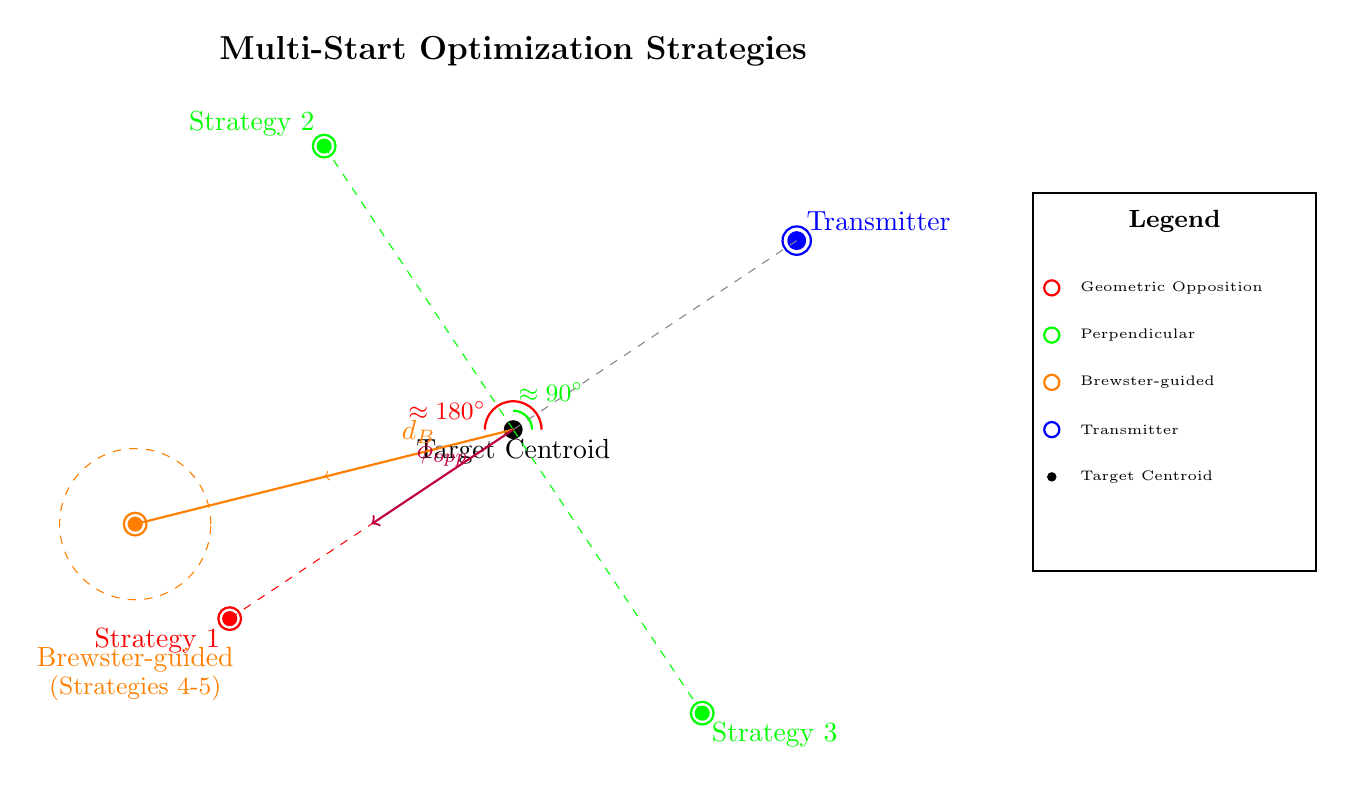
\begin{tikzpicture}[scale=1.2]

% Centro de targets
\coordinate (Center) at (0, 0);
\fill[black] (Center) circle (0.1);
\node[below] at (Center) {Target Centroid};

% Transmisor
\coordinate (Tx) at (3, 2);
\draw[blue, thick] (Tx) circle (0.15);
\fill[blue] (Tx) circle (0.1);
\node[above right, blue] at (Tx) {Transmitter};

% Línea Tx-Center
\draw[gray, dashed] (Tx) -- (Center);

% Estrategia 1: Posición opuesta
\coordinate (Rx1) at (-3, -2);
\draw[red, thick] (Rx1) circle (0.12);
\fill[red] (Rx1) circle (0.08);
\node[below left, red] at (Rx1) {Strategy 1};
\draw[red, dashed] (Center) -- (Rx1);

% Estrategia 2: Perpendicular
\coordinate (Rx2) at (-2, 3);
\draw[green, thick] (Rx2) circle (0.12);
\fill[green] (Rx2) circle (0.08);
\node[above left, green] at (Rx2) {Strategy 2};
\draw[green, dashed] (Center) -- (Rx2);

% Estrategia 3: Perpendicular opuesta
\coordinate (Rx3) at (2, -3);
\draw[green, thick] (Rx3) circle (0.12);
\fill[green] (Rx3) circle (0.08);
\node[below right, green] at (Rx3) {Strategy 3};
\draw[green, dashed] (Center) -- (Rx3);

% Estrategia 4-5: Brewster-guided (con zona de aleatoriedad)
\coordinate (RxBrewster) at (-4, -1);
\draw[orange, thick] (RxBrewster) circle (0.12);
\fill[orange] (RxBrewster) circle (0.08);

% Zona de aleatoriedad alrededor del punto Brewster
\draw[orange, dashed] (RxBrewster) circle (0.8);
\node[below, orange] at (-4, -2.2) {Brewster-guided};
\node[below, orange, font=\small] at (-4, -2.5) {(Strategies 4-5)};

% Ángulo de Brewster ilustrativo
\draw[orange, thick] (Center) -- (RxBrewster);
\draw[orange, ->] (Center) -- (-2, -0.5) node[midway, above] {$d_B$};

% Azimut opuesto
\draw[purple, thick, ->] (Center) -- (-1.5, -1) node[midway, above] {$\phi_{opp}$};

% Ángulo bistático para Strategy 1
\draw[red, thick] (Center) ++(0.3, 0) arc (0:180:0.3);
\node[red, font=\small] at (-0.7, 0.2) {$\approx 180^\circ$};

% Ángulos bistáticos para perpendiculares
\draw[green, thick] (Center) ++(0.2, 0) arc (0:90:0.2);
\node[green, font=\small] at (0.4, 0.4) {$\approx 90^\circ$};

% Etiquetas adicionales
\node[font=\large\bfseries] at (0, 4) {Multi-Start Optimization Strategies};

% Leyenda
\begin{scope}[shift={(5.5, 1)}]
    \draw[thick] (0, 1.5) rectangle (3, -2.5);
    \node[font=\small\bfseries] at (1.5, 1.2) {Legend};
    
    \draw[red, thick] (0.2, 0.5) circle (0.08);
    \node[font=\tiny, right] at (0.4, 0.5) {Geometric Opposition};
    
    \draw[green, thick] (0.2, 0) circle (0.08);
    \node[font=\tiny, right] at (0.4, 0) {Perpendicular};
    
    \draw[orange, thick] (0.2, -0.5) circle (0.08);
    \node[font=\tiny, right] at (0.4, -0.5) {Brewster-guided};
    
    \draw[blue, thick] (0.2, -1) circle (0.08);
    \node[font=\tiny, right] at (0.4, -1) {Transmitter};
    
    \fill[black] (0.2, -1.5) circle (0.05);
    \node[font=\tiny, right] at (0.4, -1.5) {Target Centroid};
\end{scope}

\end{tikzpicture}
\end{document}}
% \includegraphics[width=0.48\textwidth]{optimization_strategies.png}
\caption{Multi-start optimization strategies for bistatic receiver positioning. Strategy 1 (red) maximizes bistatic angle through geometric opposition. Strategies 2-3 (green) provide perpendicular positioning. Strategies 4-5 (orange) use pseudo-Brewster angle-guided positioning.}
\label{fig:optimization_strategies}
\end{figure}

The homogeneous reflectivity assumption is intentionally adopted to isolate the effect of acquisition geometry. This controlled setting allows a direct evaluation of electromagnetic coupling without conflating geometry effects with target-dependent scattering variability.

\subsection{Enhanced Data Quality for Tomographic Processing}

Pseudo-Brewster-guided acquisition is expected to improve tomographic processing by increasing acquisition-domain SNR ($\mathrm{SNR} \propto P_r$). Data can be reconstructed with standard time-domain backprojection and absolute radiometric calibration (corner reflectors), enabling direct comparison with baseline geometries under consistent processing conditions. Although improved coupling should favor detectability and contrast, direct gains in penetration depth and tomographic fidelity still require controlled inversion experiments.

In practical SAR systems, increased received power improves robustness to oscillator phase noise, residual motion errors, navigation uncertainty, and clutter-limited conditions, thereby enhancing detection reliability in attenuating media.

\section{Results and Analysis}

We quantitatively evaluate the pseudo-Brewster-guided framework using received power at the bistatic receiver as the coupling-efficiency metric at 400~MHz, comparing Brewster-guided, perpendicular, and opposite strategies.

\subsection{Flight Planning Validation}

The QGIS plugin successfully computed pseudo-Brewster-angle ranges for different moisture conditions and generated viable flight plans. Integration with the RD350 drone control software was established, enabling mission execution based on the generated plans.

The optimization framework consistently identifies receiver positions associated with higher received power. Table~\ref{tab:optimization_results} summarizes the performance comparison between different initialization strategies.

\begin{table}[hbt]
\centering
\caption{Bistatic Receiver Optimization Strategy Performance Comparison at 400 MHz}
\label{tab:optimization_results}
\setlength{\tabcolsep}{4pt} % default is 6pt
\small
\begin{tabular}{lrrrr}
\toprule
\textbf{Strategy} & \textbf{Avg} & \textbf{Max} & \textbf{Min} & \textbf{Improv. (\%)} \\
\midrule
Brewster & -70.11 & -67.82 & -75.22 & 0.00 \\
Perpendicular & -72.99 & -71.68 & -77.44 & 4.11 \\
Opposite & -72.30 & -71.23 & -76.76 & 3.13 \\
\bottomrule
\end{tabular}
\end{table}

Results are averaged over multiple initialization seeds, and the consistency of the observed gain confirms that the improvement is systematic rather than incidental.

The simulations were conducted at a carrier frequency of 400 MHz (UHF band), corresponding to a wavelength of 0.75 m in air. This frequency selection represents a practical compromise between penetration depth and spatial resolution for subsurface sensing applications. All power measurements are expressed in dBm (decibels relative to 1 mW), with 0 dBm corresponding to 1 mW, providing standardized power-level references for comparison across different optimization strategies.

Brewster-guided positioning achieves the highest average received power of $-70.11 \,\mathrm{dBm}$, indicating a consistent improvement in electromagnetic coupling efficiency at the subsurface interface under the simulated conditions. In contrast, the perpendicular and opposite strategies yield lower average received powers of $-72.99, \mathrm{dBm}$ and $-72.30, \mathrm{dBm}$, respectively, consistent with higher reflection losses. These results support the use of pseudo-Brewster-angle optimization to enhance signal transmission efficiency at the interface under the simulated scenarios considered here.

\subsection{Electromagnetic Performance}

Because reflectivity is minimized near the pseudo-Brewster angle, the optimized geometry increases interface transmittance. Coverage can be quantified as $C(\eta)=|\mathcal{V}|^{-1}\sum_v\mathbf{1}\{P_r(v)\ge\eta\}$, where $P_r(v)$ denotes the received power from voxel $v$ evaluated via Eq.~\ref{eq:bistatic_radar}, with complementary blind-spot ratio $B(\eta)=1-C(\eta)$ for a detection threshold $\eta$. This formulation links geometry-level power improvements to volumetric detectability analysis and provides a direct bridge to future reconstruction validation. While full voxel-level coverage evaluation is part of ongoing work, the current results demonstrate strategy-level power improvements consistent with expected gains in volumetric detectability.

These definitions enable reproducible comparison across acquisition strategies under consistent detection thresholds.

%\subsection{Tomographic Reconstruction Quality}

Higher coupling is expected to improve tomographic sensitivity to dielectric contrasts; an approximate depth relation is $\Delta z \approx \ln F/(2\alpha)$, where $F$ is the power-gain factor and $\alpha$ is attenuation. This remains model-based pending field validation. Figure~\ref{fig:bistatic_3d_config} shows the optimized 3D geometry.

\begin{figure}[!htb]
\centering
\includegraphics[width=1\columnwidth]{bistatic_configuration_3d.png}
\caption{Optimized bistatic radar 3D configuration showing transmitter spiral (blue), receiver positions (orange), and subsurface targets (red) with air-ground interface.}
\label{fig:bistatic_3d_config}
\end{figure}

Figure~\ref{fig:bistatic_comparison} compares received power across strategies and highlights the consistent advantage of Brewster-guided initialization.

\begin{figure}[H]
\centering
\includegraphics[width=0.4\textwidth]{fig5.png}
\caption{Received power comparison between different bistatic optimization strategies showing the performance advantage of Brewster-guided positioning over perpendicular and opposite approaches across multiple simulation scenarios.}
\label{fig:bistatic_comparison}
\end{figure}

\section{Discussion and Future Work}

The main contribution of this work is a unified workflow that combines electromagnetic optimization via pseudo-Brewster angles with practical mission planning for bistatic SAR. The framework integrates optimization algorithms and can support future machine-learning-based processing for subsurface sensing.

Current limitations include: (i) a simulation-only scope, since reconstruction-level metrics such as CNR, PSF, and localization error have not yet been evaluated; (ii) permittivity sensitivity, because pseudo-Brewster guidance depends on soil dielectric properties and mismatches between assumed and actual permittivity may affect optimization robustness; and (iii) a single-interface model, since the first-order Fresnel criterion does not fully capture volumetric heterogeneity, layered media, and multiple internal reflections. Future work will address:

\begin{itemize}
\item Controlled field campaigns with the RD350 platform under known dielectric conditions
\item Backprojection-based reconstruction comparison (Brewster-guided vs.\ baseline) with quantitative metrics
\item Permittivity sensitivity analysis: propagation of $\delta\varepsilon_r$ uncertainty through the optimization pipeline
\item Platform motion and noise perturbation tests to verify power advantage under realistic conditions
\item Multi-frequency extensions and polarimetric integration
\end{itemize}

Overall, the proposed system provides a framework for optimizing bistatic radar deployment in subsurface sensing applications.
\section{Conclusions}

This work presented a pseudo-Brewster-angle-guided bistatic SAR framework for subsurface sensing, integrating electromagnetic transmission theory, receiver-position optimization, and flight-planning constraints. Simulation results at 400 MHz show that the Brewster-guided configuration achieved the highest average received power, reaching $-70.11$~dBm, compared with $-72.99$~dBm for the perpendicular configuration and $-72.30$~dBm for the opposite configuration, indicating consistent acquisition-domain gains under the evaluated conditions. Although still limited to simulation-level validation, the framework offers a practical basis for coupling-aware mission planning in drone-borne bistatic SAR systems. Future work will focus on field experiments, reconstruction-level evaluation, and sensitivity analysis under realistic dielectric, motion, and noise uncertainties.

\section *{Acknowledgment}
This research was also funded by the National Council for Scientific and Technological Development (CNPq), grants 141109/2023-8 (Eder) and 314539/2023-9 (HEHF), and by the São Paulo Research Foundation (FAPESP), projects 2021/11380-5 (CPTEn), 2021/00199-8 (SMARTNESS),
2022/11596-0 (EMU) and 2024/15524-0 (NSFC).

\begin{thebibliography}{99}

\bibitem{daniels_gpr}
D.~J.~Daniels, \emph{Ground Penetrating Radar}, 2nd~ed. New York, NY, USA: IEEE Press, 2004.

\bibitem{Soil}
G.~C.~Oré~Huacles \emph{et~al.}, ``Soil moisture monitoring for precision agriculture via drone-borne multi-band synthetic aperture radar,'' in \emph{Proc. PIERS}, 2025.

\bibitem{cherniakov_bistatic}
M.~Cherniakov, \emph{Bistatic Radar: Principles and Practice}. Hoboken, NJ, USA: Wiley, 2007.

\bibitem{mcmichael_brewster}
I.~McMichael, ``A note on the Brewster angle in lossy dielectric media,'' U.S. Army RDECOM CERDEC NVESD, Fort Belvoir, VA, USA, Tech. Rep. RDER-NV-TR-267, Oct.~2010.

\bibitem{ore_soil_moisture}
G.~Oré, J.~Yepes, J.~A.~Góes, L.~P.~Oliveira, B.~Teruel, and H.~E.~Hernandez-Figueroa,
``Soil moisture estimation of bare and vegetation-covered areas using P/L/C-band SAR,''
unpublished manuscript, Univ. of Campinas, Campinas, Brazil, Dec. 2024.

\bibitem{willis_bistatic}
N.~J.~Willis and H.~D.~Griffiths, \emph{Advances in Bistatic Radar}. Raleigh, NC, USA: SciTech Publishing, 2007.

\bibitem{born_optics}
M.~Born and E.~Wolf, \emph{Principles of Optics}, 7th~ed. Cambridge, U.K.: Cambridge Univ. Press, 1999.

\bibitem{taflove_fdtd}
A.~Taflove and S.~C.~Hagness, \emph{Computational Electrodynamics: The Finite-Difference Time-Domain Method}, 3rd~ed. Boston, MA, USA: Artech House, 2005.

\bibitem{dann_architecture}
Y.~Ganin \emph{et~al.}, ``Domain-adversarial training of neural networks,'' \emph{J. Mach. Learn. Res.}, vol.~17, no.~1, pp.~2096--2030, 2016.

\bibitem{sar_processing}
I.~G.~Cumming and F.~H.~Wong, \emph{Digital Processing of Synthetic Aperture Radar Data}. Boston, MA, USA: Artech House, 2005.

\bibitem{Water}
L.~P.~Oliveira \emph{et~al.}, ``Subsurface water leakage detection using P-band SAR imaging: A controlled experiment,'' in \emph{Proc. IGARSS}, 2025.

\bibitem{UAV}
P.~M.~O.~Costa \emph{et~al.}, ``UAV-borne synthetic aperture radar system for detection of buried petroleum pipelines,'' in \emph{Proc. IGARSS}, 2025.

\bibitem{Subsurface}
D.~Munch \emph{et~al.}, ``SAR-based subsurface tomography: An iron mine case study,'' in \emph{Proc. IGARSS}, 2025.

\bibitem{Burrows}
G.~C.~Oré~Huacles \emph{et~al.}, ``Localization of beaver burrows by P-band SAR tomography,'' in \emph{Proc. PIERS}, 2025.

\bibitem{Iron}
G.~C.~Oré~Huacles \emph{et~al.}, ``Iron mine survey based on drone-borne tomographic SAR system,'' in \emph{Proc. PIERS}, 2025.

\end{thebibliography}


\end{document}